\documentclass{article}
\usepackage{url}
\usepackage{fancyhdr}
\usepackage{extramarks}
\usepackage{amsmath}
\usepackage{amsthm}
\usepackage{amsfonts}
\usepackage{tikz}
\usetikzlibrary{3d}
\usepackage[plain]{algorithm}
\usepackage{algpseudocode}
\usepackage{braket}
\usepackage{enumerate}
\usepackage{paralist}
\usepackage{hyperref}
%
% Basic Document Settings
%
\topmargin=-0.45in
\evensidemargin=0in
\oddsidemargin=0in
\textwidth=6.5in
\textheight=9.0in
\headsep=0.25in
\linespread{1.1}
\pagestyle{fancy}
\lhead{Habib University}
\chead{\hmwkClass, \hmwkTitle}
\rhead{\firstxmark}
\lfoot{\lastxmark}
\cfoot{\thepage}
\renewcommand\headrulewidth{0.4pt}
\renewcommand\footrulewidth{0.4pt}
\setlength\parindent{0pt}
%
% Create Problem Sections
%
\newcommand{\enterProblemHeader}[1]{
\nobreak\extramarks{}{Problem \arabic{#1} continued on next page\ldots}
\nobreak{}
\nobreak\extramarks{Problem \arabic{#1} (continued)}{Problem \arabic{#1}
continued on next page\ldots}\nobreak{}
}
\newcommand{\exitProblemHeader}[1]{
\nobreak\extramarks{Problem \arabic{#1} (continued)}{Problem \arabic{#1}
continued on next page\ldots}\nobreak{}
\stepcounter{#1}
\nobreak\extramarks{Problem \arabic{#1}}{}\nobreak{}
}
\setcounter{secnumdepth}{0}
\newcounter{partCounter}
\newcounter{homeworkProblemCounter}
\setcounter{homeworkProblemCounter}{1}
\nobreak\extramarks{Problem \arabic{homeworkProblemCounter}}{}\nobreak{}
%
% Homework Problem Environment
%
% This environment takes an optional argument. When given, it will adjust the
% problem counter. This is useful for when the problems given for your
% assignment aren't sequential. See the last 3 problems of this template for an
% example.
%
\newenvironment{homeworkProblem}[1][-1]{
\ifnum#1>0
\setcounter{homeworkProblemCounter}{#1}
\fi
\section{Problem \arabic{homeworkProblemCounter}}
\setcounter{partCounter}{1}
\enterProblemHeader{homeworkProblemCounter}
}{
\exitProblemHeader{homeworkProblemCounter}
}
%
% Homework Details
% - Title
% - Due date
% - Class
% - Section/Time
% - Instructor
% - Author
%
\newcommand{\hmwkTitle}{Homework\ \#3}
\newcommand{\hmwkDueDate}{November 24, 2026, 11.59pm}
\newcommand{\hmwkClass}{CS 314/PHYS 300: Quantum Computing}
\newcommand{\hmwkClassInstructor}{Dr. Faisal Alvi}
\newcommand{\hmwkAuthorName}{\textbf{Sameez Sarfaraz Sajwani (ss09212)} \and \textbf{Hassan Akhter (ha10609)}}
%
% Title Page
%
\title{
\vspace{2in}
\textmd{\textbf{\hmwkClass:\\ \hmwkTitle}}\\
\normalsize\vspace{0.1in}\small{\hmwkClassInstructor}\\
\normalsize\vspace{0.1in}\small{Due\ on\ \hmwkDueDate}\\
\vspace{3in}
}
\author{\hmwkAuthorName}
\date{}
\renewcommand{\part}[1]{\textbf{\large Part \Alph{partCounter}}
\stepcounter{partCounter}\\}
%
% Various Helper Commands
%
% Useful for algorithms
\newcommand{\alg}[1]{\textsc{\bfseries \footnotesize #1}}
% For derivatives
\newcommand{\deriv}[1]{\frac{\mathrm{d}}{\mathrm{d}x} (#1)}
% For partial derivatives
\newcommand{\pderiv}[2]{\frac{\partial}{\partial #1} (#2)}
% Integral dx
\newcommand{\dx}{\mathrm{d}x}
% Alias for the Solution section header
\newcommand{\solution}{\textbf{\large Solution}}
% Probability commands: Expectation, Variance, Covariance, Bias
\newcommand{\E}{\mathrm{E}}
\newcommand{\Var}{\mathrm{Var}}
\newcommand{\Cov}{\mathrm{Cov}}
\newcommand{\Bias}{\mathrm{Bias}}

\begin{document}
\maketitle
\pagebreak

\begin{homeworkProblem}
(15 points) [\textbf{Grover's Algorithm - States}] In the version of Grover's
Algorithm that we studied in the class (where our initial state was $\ket{\psi}$ as
a uniform superposition of all states) we used:
\begin{itemize}
\item an oracle `$O$' to invert the sign of the required state.
\item a Grover Diffusion Operator `$G$' denoted by $2\ket{\psi}\bra{\psi} -
I$ to amplify the amplitude of the inverted state.
\end{itemize}
\begin{enumerate}[(a)]
\item (10 points) Show that the Grover's Diffusion Operator `$G$'
\begin{center}
$2\ket{\psi}\bra{\psi} - I$
\end{center}
is equivalent to
\begin{center}
$H^{\otimes n} (2\ket{0}\bra{0} - I) H^{\otimes n}$.
\end{center}
\item (5 points) Write a Qiskit function that simulates the Grover Diffusion
Operator for 5 qubits. Test your function with various inputs.
\end{enumerate}
\end{homeworkProblem}

\solution

\begin{enumerate}[(a)]
    \item We can prove the above mentioned equivalence as follows:
    \begin{itemize}
        \item We start with the expression $H^{\otimes n} (2 \ket{0^n} \bra{0^n} - \mathbb{I}) H^{\otimes n}$.
        \item Distributing $H^{\otimes n}$ on the left, we get $(2 H^{\otimes n} \ket{0^n}\bra{0^n} - H^{\otimes n}\mathbb{I}) H^{\otimes n}$.
        \item By definition, $\ket{\psi}$ is the uniform superposition of all possible $n-$qubits states, therefore $H^{\otimes n}\ket{0^n} = \ket{\psi}$. So now our expression becomes $(2 \ket{\psi}\bra{0^n} - H^{\otimes n}\mathbb{I})H^{\otimes n}$.
        \item since $\mathbb{I}U = U\mathbb{I} = U$ for any matrix $U$ of compatible dimension, our expression now simplifies to $(2 \ket{\psi}\bra{0^n} - H^{\otimes n}) H^{\otimes n}$.
        \item distributing $H^{\otimes n}$ from the right, we get $2\ket{\psi}\bra{0^n}H^{\otimes n} - H^{\otimes n}H^{\otimes n}$.
        \item As $\ket{\psi} = H^{\otimes n}\ket{0^n}$, taking the conjugate-transpose gives us $\bra{\psi} = \bra{0} H^{\otimes n}$. Now, our expression becomes $2\ket{\psi}\bra{\psi} - H^{\otimes n}H^{\otimes n}$
        \item using the mixed-product property of tensors, we get $2\ket{\psi}\bra{\psi} - (HH)^{\otimes n}$. But since $H$ is its own conjugate-transpose, we have $HH = \mathbb{I}$. So we get $2\ket{\psi}\bra{\psi} - \mathbb{I}^{\otimes n} = 2\ket{\psi}\bra{\psi} - \mathbb{I}$ 
    \end{itemize}
    $\qed$ Q.E.D.

    \item
    Note that all the three test cases randomly select one of the $32$ possible states and flip its sign to fully demonstrate the effect of the diffusion operator. The full setup and results can be seen \href{https://colab.research.google.com/drive/11P-5j1ke_xIk-jOb2NPHdzISqHc27nK3?usp=sharing}{here}
\end{enumerate}

\newpage
\begin{homeworkProblem} (10 points) [\textbf{Grover's Algorithm - Sample Run -
Adapted from Cambridge University Course on Quantum Computation]
\textit{https://www.cl.cam.ac.uk/teaching/exams/pastpapers/y2023p8q11.pdf}}]
\vspace{5pt}
Let there be a database containing 32 elements, indexed by the binary numbers 00000
to 11111. A single element 00110 is marked.
\begin{enumerate}[(a)]
\item (3 points) If Grover’s search algorithm is applied to find the marked
element, what should the initial state be set to, and what is the state after a
single Grover iterate has been applied?
\item (4 points) To find the marked element with maximum probability requires
\textit{N} iterates in total. What is the value of \textit{N}, and what is the
probability of correctly finding the marked element? Show the complete working at
how did you arrive at the value of probability.
\item (3 points) If the algorithm is instead run with 3\textit{N} iterates in
total, what is the probability of correctly finding the marked element? Comment on
your answer.
\end{enumerate}
\end{homeworkProblem}

\solution

\begin{enumerate}[(a)]
    \item
    a search space of $32$ elements can be represented in exactly $5$ qubits, as $32 = 2^5$. The initial state must be a uniform superposition of all $32$ states, which can be obtained by taking $\ket{00000}$ and applying the $H$-gate to all 5. This generates our starting state as
    \[
    \ket{s} = \frac{1}{\sqrt{32}}
              \begin{bmatrix}
                  1 \\
                  1 \\
                  \cdots \\
                  1
              \end{bmatrix}
    \]

    A single iteration of the Grover's search algorithm is made up of 2 steps: applying the oracle, followed by the diffusion operator. The oracle and diffusion matrix for our current setup would be of order $32 \times 32$. However, we can simplify the problem as follows: \\
    Let $\ket{\alpha}, \ket{\beta}$ be two special qubits, representing the marked and unmarked states respectively. In our case, $\ket{\alpha} = \ket{00110}$ and $\ket{\beta} = \frac{1}{\sqrt{31}} \sum_{k=0}^{31}(1 - \delta_{k6})\ket{k}$ where $\delta_{ij}$ is the Kronecker-delta. Ensuring normalization, we get $\ket{s} = \sqrt{\frac{1}{32}}\ket{\alpha} + \sqrt{\frac{31}{32}}\ket{\beta}$.

    We now define a $2D$ plane where the unmarked state $\ket{\beta}$ lies on the $x$-axis and the marked state $\ket{\alpha}$ lies on the $y$-axis. Then, $\ket{s} = \sin(\frac{\theta}{2})\ket{\alpha} + \cos(\frac{\theta}{2})\ket{\beta}$. Comparing the two definitions of $\ket{s}$, we get $\theta = 2\arcsin(\frac{1}{\sqrt{32}})$. This will become useful in the later parts.

    The Oracle $U_f$ only flips the phase of the marked state, and leaves the unmarked state unchanged. Therefore
    \[
    U_f = \begin{bmatrix}
        -1  &   0   \\
        0   &   1
    \end{bmatrix}
    \]
    The Diffusion operator $G = 2\ket{s}\bra{s} - \mathbb{I}$. Putting in the value for $\ket{s}$, we get
    \[
    G = 2 \begin{bmatrix}
        \frac{1}{\sqrt{32}} \\
        \sqrt{\frac{31}{32}}
    \end{bmatrix} \begin{bmatrix}
        \frac{1}{\sqrt{32}} &   \sqrt{\frac{31}{32}}
    \end{bmatrix} - \begin{bmatrix}
        1   &   0   \\
        0   &   1
    \end{bmatrix} = \frac{1}{16} \begin{bmatrix}
        -15 &   \sqrt{31}   \\
        \sqrt{31}   &   15
    \end{bmatrix}
    \]

    A single iteration of Grover's algorithm involves applying the Oracle, followed by the Diffusion. That is, any input qubit goes through the transformation of $\ket{\psi} \longrightarrow U_f\ket{\psi} \longrightarrow GU_f\ket{\psi}$. In our case,
    \[
    GU_f = \frac{1}{16} \begin{bmatrix}
        -15 &   \sqrt{31}   \\
        \sqrt{31}   &   15
    \end{bmatrix} \begin{bmatrix}
        -1  &   0   \\
        0   &   1
    \end{bmatrix} = \frac{1}{16} \begin{bmatrix}
        15  &   \sqrt{31}   \\
        -\sqrt{31}  &   15
    \end{bmatrix}
    \]

    Applying $GU_f$ to our qubit $\ket{s}$, we get $\frac{23\sqrt{2}}{64}\ket{\alpha} + \frac{7\sqrt{62}}{64}\ket{\beta}$.

    Therefore, the probability of measuring $\ket{\alpha}$ is $\vert\frac{23\sqrt{2}}{64}\vert^2 \approx 25.83\%$

    \item
    By reducing the $2^n$-dimensional space (where $n$ is the number of qubits) down to a $2D$ plane in terms of $\ket{\alpha}, \ket{\beta}$, we have mapped each iteration of Grover's algorithm to a simple rotation in the $xy$-plane. Repeated application of $GU_f$ transforms our original $\ket{s}$ into $\sin(\frac{(2N+1)\theta}{2})\ket{\alpha} + \cos(\frac{(2N+1)\theta}{2})\ket{\beta}$. We want $N$ such that the probability of measuring $\ket{\alpha}$ is maximum. This happens when the $\arg$ within the $\sin$ function is as close to $\frac{\pi}{2}$ as possible. Therefore,
    \[
    \frac{(2N+1)\theta}{2} \approx \frac{\pi}{2}
    \]
    \[
    (2N+1)\theta \approx \pi
    \]
    \[
    2N+1 \approx \frac{\pi}{\theta}
    \]
    \[
    2N \approx \frac{\pi}{\theta} - 1 = \frac{\pi}{\theta} - \frac{\theta}{\theta} = \frac{\pi-\theta}{\theta}
    \]
    \[N \approx \frac{\pi-\theta}{2\theta}\]
    We know for sure that $N < \frac{\pi-\theta}{\theta}$ will always undershoot. So instead, we take $N = \lceil\frac{\pi-\theta}{\theta}\rceil$. From the previous part, we know that $\theta = 2\arcsin(\frac{1}{\sqrt{32}})$. Putting the value in, we get $N = \lceil{3.916}\rceil = 4$.

    From above, we know that the amplitude of measuring $\ket{\alpha}$ is $\sin(\frac{(2N+1)\theta}{2})$. Putting in the values for $N, \theta$ yields $\approx 0.9995$. Therefore, the probability of measuring $\ket{\alpha}$ is $\vert\sin(\frac{(2N+1)\theta}{2})\vert^2 \approx 0.9991$

    \item
    replacing $N = 4$ with $3N = 12$ in the above expression, we get the probability of measuring $\alpha$ to be $\vert\sin(\frac{(6N+1)\theta}{2})\vert^2 \approx 0.929$.

    Since we went beyond the optimal iterations, the result that we achieve is also sub-optimal.
\end{enumerate}

\newpage
\begin{homeworkProblem} (10 points) \textbf{[Eigenvalues and Eigenvectors]} Find
the Eigenvalues and Eigenvectors of:
\begin{enumerate} [(a)]
\item (4 points) The `$X$' (or the not) quantum operator given by
$\begin{bmatrix}
0 & 1 \\
1 & 0
\end{bmatrix}.$
\item (6 points) The `$H$' (or the Hadamard) Operator given by: $
\begin{bmatrix}
1/\sqrt{2} & 1/\sqrt{2} \\
1/\sqrt{2} & -1/\sqrt{2}
\end{bmatrix}.$
\end{enumerate}
The Eigenvalues of a square matrix $A$ can be calculated by solving for the
eigenvalues `$\lambda$' in the equation `$det(A - \lambda I) = 0$', and then
solving for the eigenvector $v$ using the equation `$(\lambda I - A)v = 0$'. Since
we are working with qubits, ensure that the norm of your eigenvectors equals to 1.
Show all your work.
\end{homeworkProblem}

\solution

\begin{enumerate}[(a)]
    \item Let $X = \begin{bmatrix} 0 & 1 \\ 1 & 0 \end{bmatrix}$. To find the eigenvalues, we solve $\det(X - \lambda I) = 0$:
    \[
    \det \left( \begin{bmatrix} 0 & 1 \\ 1 & 0 \end{bmatrix} - \begin{bmatrix} \lambda & 0 \\ 0 & \lambda \end{bmatrix} \right) = \det \begin{bmatrix} -\lambda & 1 \\ 1 & -\lambda \end{bmatrix} = 0
    \]
    \[
    (-\lambda)(-\lambda) - (1)(1) = 0 \implies \lambda^2 - 1 = 0 \implies \lambda = \pm 1
    \]
    Thus, the eigenvalues are $\lambda_1 = 1$ and $\lambda_2 = -1$.

    \textbf{For $\lambda_1 = 1$:}
    We solve $(\lambda_1 I - X)v_1 = 0$ where $v_1 = \begin{bmatrix} x \\ y \end{bmatrix}$:
    \[
    \begin{bmatrix} 1 & -1 \\ -1 & 1 \end{bmatrix} \begin{bmatrix} x \\ y \end{bmatrix} = \begin{bmatrix} 0 \\ 0 \end{bmatrix} \implies x - y = 0 \implies x = y
    \]
    Choosing $x = 1$ gives $y = 1$, so the unnormalized eigenvector is $\begin{bmatrix} 1 \\ 1 \end{bmatrix}$. Normalizing to unit length ($\|v_1\| = \sqrt{1^2 + 1^2} = \sqrt{2}$):
    \[
    v_1 = \frac{1}{\sqrt{2}} \begin{bmatrix} 1 \\ 1 \end{bmatrix} = \ket{+}
    \]

    \textbf{For $\lambda_2 = -1$:}
    We solve $(\lambda_2 I - X)v_2 = 0$ where $v_2 = \begin{bmatrix} x \\ y \end{bmatrix}$:
    \[
    \begin{bmatrix} -1 & -1 \\ -1 & -1 \end{bmatrix} \begin{bmatrix} x \\ y \end{bmatrix} = \begin{bmatrix} 0 \\ 0 \end{bmatrix} \implies -x - y = 0 \implies y = -x
    \]
    Choosing $x = 1$ gives $y = -1$, so the unnormalized eigenvector is $\begin{bmatrix} 1 \\ -1 \end{bmatrix}$. Normalizing to unit length ($\|v_2\| = \sqrt{1^2 + (-1)^2} = \sqrt{2}$):
    \[
    v_2 = \frac{1}{\sqrt{2}} \begin{bmatrix} 1 \\ -1 \end{bmatrix} = \ket{-}
    \]

    \item Let $H = \frac{1}{\sqrt{2}} \begin{bmatrix} 1 & 1 \\ 1 & -1 \end{bmatrix}$. To find the eigenvalues, we solve $\det(H - \lambda I) = 0$:
    \[
    \det \begin{bmatrix} \frac{1}{\sqrt{2}} - \lambda & \frac{1}{\sqrt{2}} \\ \frac{1}{\sqrt{2}} & -\frac{1}{\sqrt{2}} - \lambda \end{bmatrix} = 0
    \]
    \[
    \left(\frac{1}{\sqrt{2}} - \lambda\right)\left(-\frac{1}{\sqrt{2}} - \lambda\right) - \left(\frac{1}{\sqrt{2}}\right)\left(\frac{1}{\sqrt{2}}\right) = 0
    \]
    \[
    \lambda^2 - \frac{1}{2} - \frac{1}{2} = 0 \implies \lambda^2 - 1 = 0 \implies \lambda = \pm 1
    \]
    Thus, the eigenvalues are $\lambda_1 = 1$ and $\lambda_2 = -1$.

    \textbf{For $\lambda_1 = 1$:}
    We solve $(\lambda_1 I - H)v_1 = 0$ where $v_1 = \begin{bmatrix} x \\ y \end{bmatrix}$:
    \[
    \begin{bmatrix} 1 - \frac{1}{\sqrt{2}} & -\frac{1}{\sqrt{2}} \\ -\frac{1}{\sqrt{2}} & 1 + \frac{1}{\sqrt{2}} \end{bmatrix} \begin{bmatrix} x \\ y \end{bmatrix} = \begin{bmatrix} 0 \\ 0 \end{bmatrix}
    \]
    From the first row:
    \[
    \left(1 - \frac{1}{\sqrt{2}}\right)x - \frac{1}{\sqrt{2}}y = 0 \implies \frac{\sqrt{2} - 1}{\sqrt{2}}x = \frac{1}{\sqrt{2}}y \implies y = (\sqrt{2} - 1)x
    \]
    (Note: multiplying the second row by $\sqrt{2}-1$ yields the exact same equation.) Setting $x = 1$ gives $y = \sqrt{2} - 1$. Computing the norm:
    \[
    \|v_1\| = \sqrt{1^2 + (\sqrt{2} - 1)^2} = \sqrt{1 + (2 - 2\sqrt{2} + 1)} = \sqrt{4 - 2\sqrt{2}}
    \]
    Dividing by $\|v_1\|$, the normalized eigenvector is:
    \[
    v_1 = \frac{1}{\sqrt{4 - 2\sqrt{2}}} \begin{bmatrix} 1 \\ \sqrt{2} - 1 \end{bmatrix}
    \]
    *(Equivalently, in trigonometric form, $v_1 = \begin{bmatrix} \cos(\pi/8) \\ \sin(\pi/8) \end{bmatrix}$.)*

    \textbf{For $\lambda_2 = -1$:}
    We solve $(\lambda_2 I - H)v_2 = 0$ where $v_2 = \begin{bmatrix} x \\ y \end{bmatrix}$:
    \[
    \begin{bmatrix} -1 - \frac{1}{\sqrt{2}} & -\frac{1}{\sqrt{2}} \\ -\frac{1}{\sqrt{2}} & -1 + \frac{1}{\sqrt{2}} \end{bmatrix} \begin{bmatrix} x \\ y \end{bmatrix} = \begin{bmatrix} 0 \\ 0 \end{bmatrix}
    \]
    From the first row:
    \[
    -\left(\frac{\sqrt{2} + 1}{\sqrt{2}}\right)x - \frac{1}{\sqrt{2}}y = 0 \implies y = -(\sqrt{2} + 1)x
    \]
    Setting $x = 1$ gives $y = -(\sqrt{2} + 1)$. Computing the norm:
    \[
    \|v_2\| = \sqrt{1^2 + (-(\sqrt{2} + 1))^2} = \sqrt{1 + (2 + 2\sqrt{2} + 1)} = \sqrt{4 + 2\sqrt{2}}
    \]
    Dividing by $\|v_2\|$, the normalized eigenvector is:
    \[
    v_2 = \frac{1}{\sqrt{4 + 2\sqrt{2}}} \begin{bmatrix} 1 \\ -(\sqrt{2} + 1) \end{bmatrix}
    \]
    *(Equivalently, in trigonometric form, $v_2 = \begin{bmatrix} -\sin(\pi/8) \\ \cos(\pi/8) \end{bmatrix}$.)*
\end{enumerate}

\newpage
\begin{homeworkProblem} (15 points) \textbf{[Inverse Quantum Fourier Transform
Using Pauli Matrices and $H$]}
\begin{enumerate}[(a)]
\item (10 points) Using the circuit for \textit{inverse} quantum fourier transform,
construct (draw) the circuit for the \textit{inverse} fourier transform for 2 bits
using the Hadamard, controlled-\textit{T} and controlled-NOT gates only. Show that
the original circuit for the inverse QFT and your circuit are equivalent.
\item (5 points) Write a Qiskit function to implement this inverse quantum fourier
transform. Run your circuit for all combinations of two qubits and show that the
output is correct.
\end{enumerate}
\end{homeworkProblem}

\solution

\begin{enumerate}[(a)]
    \item For 2 qubits $\ket{q_0 q_1}$ (where $q_0$ is the most significant bit), the standard 2-qubit inverse Quantum Fourier Transform ($\text{QFT}_2^\dagger$) consists of:
    \begin{enumerate}
        \item A SWAP gate between $q_0$ and $q_1$ (reversing the qubit order).
        \item A Hadamard gate $H$ on $q_0$.
        \item A controlled-$R_2^\dagger$ gate (where $R_2 = S = \begin{bmatrix} 1 & 0 \\ 0 & i \end{bmatrix}$, so $R_2^\dagger = S^\dagger = \begin{bmatrix} 1 & 0 \\ 0 & -i \end{bmatrix}$) controlled by $q_0$ acting on $q_1$.
        \item A Hadamard gate $H$ on $q_1$.
    \end{enumerate}

    To construct this circuit using \textbf{only} $H$, controlled-$T$ ($CT$), and CNOT gates:
    \begin{itemize}
        \item \textbf{SWAP decomposition:} A standard SWAP gate between $q_0$ and $q_1$ is identically decomposed into three alternating CNOT gates: $\text{CNOT}_{0,1} \cdot \text{CNOT}_{1,0} \cdot \text{CNOT}_{0,1}$.
        \item \textbf{Controlled-$R_2^\dagger$ decomposition:} Since $T = \begin{bmatrix} 1 & 0 \\ 0 & e^{i\pi/4} \end{bmatrix}$ and $e^{i 2\pi} = 1$, we have:
        \[
        T^6 = \begin{bmatrix} 1 & 0 \\ 0 & e^{i 6\pi/4} \end{bmatrix} = \begin{bmatrix} 1 & 0 \\ 0 & e^{i 3\pi/2} \end{bmatrix} = \begin{bmatrix} 1 & 0 \\ 0 & -i \end{bmatrix} = S^\dagger = R_2^\dagger
        \]
        Therefore, a controlled-$S^\dagger$ gate is equivalent to applying six consecutive controlled-$T$ gates ($CT^6$).
    \end{itemize}

    \textbf{Decomposed 2-Qubit $\text{QFT}^\dagger$ Circuit:}
    \begin{center}
    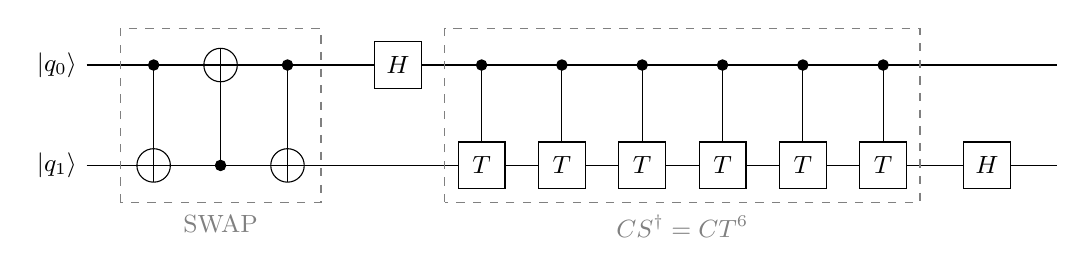
\begin{tikzpicture}[scale=0.85, every node/.style={font=\small}]
        % Wires
        \draw (0,1.5) -- (14.5,1.5);
        \draw (0,0) -- (14.5,0);
        \node[left] at (0,1.5) {$\ket{q_0}$};
        \node[left] at (0,0) {$\ket{q_1}$};

        % CNOT 1 (control q0, target q1)
        \filldraw (1.0,1.5) circle (2.2pt);
        \draw (1.0,1.5) -- (1.0,-0.25);
        \draw (1.0,0) circle (0.25);

        % CNOT 2 (control q1, target q0)
        \filldraw (2.0,0) circle (2.2pt);
        \draw (2.0,0) -- (2.0,1.75);
        \draw (2.0,1.5) circle (0.25);

        % CNOT 3 (control q0, target q1)
        \filldraw (3.0,1.5) circle (2.2pt);
        \draw (3.0,1.5) -- (3.0,-0.25);
        \draw (3.0,0) circle (0.25);

        % Dashed box around SWAP
        \draw[dashed, gray] (0.5,-0.55) rectangle (3.5,2.05);
        \node[below, gray] at (2.0,-0.6) {SWAP};

        % H on q0
        \draw[fill=white] (4.3,1.15) rectangle (5.0,1.85);
        \node at (4.65,1.5) {$H$};

        % Six Controlled-T gates (control q0, target q1)
        \foreach \x [count=\i] in {5.9, 7.1, 8.3, 9.5, 10.7, 11.9} {
            \filldraw (\x,1.5) circle (2.2pt);
            \draw (\x,1.5) -- (\x,0.35);
            \draw[fill=white] (\x-0.35,-0.35) rectangle (\x+0.35,0.35);
            \node at (\x,0) {$T$};
        }
        \draw[dashed, gray] (5.35,-0.55) rectangle (12.45,2.05);
        \node[below, gray] at (8.9,-0.6) {$CS^\dagger = CT^6$};

        % H on q1
        \draw[fill=white] (13.1,-0.35) rectangle (13.8,0.35);
        \node at (13.45,0) {$H$};
    \end{tikzpicture}
    \end{center}

    \textbf{Proof of Equivalence:}
    We verify equivalence by computing the $4 \times 4$ unitary matrix of the constructed circuit and comparing it against the canonical $\text{QFT}_2^\dagger$ matrix. Using standard big-endian ordering ($\ket{q_0 q_1}$):
    \begin{enumerate}
        \item The three CNOT gates perform the SWAP operation:
        \[
        U_{\text{SWAP}} = \text{CNOT}_{0,1}\text{CNOT}_{1,0}\text{CNOT}_{0,1} = \begin{bmatrix} 1 & 0 & 0 & 0 \\ 0 & 0 & 1 & 0 \\ 0 & 1 & 0 & 0 \\ 0 & 0 & 0 & 1 \end{bmatrix}
        \]
        \item Applying $H \otimes I$ acts as $H$ on $q_0$ and $I$ on $q_1$:
        \[
        H \otimes I = \frac{1}{\sqrt{2}} \begin{bmatrix} 1 & 0 & 1 & 0 \\ 0 & 1 & 0 & 1 \\ 1 & 0 & -1 & 0 \\ 0 & 1 & 0 & -1 \end{bmatrix}
        \]
        \item Applying $CT$ six times applies a phase of $(e^{i\pi/4})^6 = e^{i 3\pi/2} = -i$ solely to the $\ket{11}$ state:
        \[
        CT^6 = \text{diag}(1, 1, 1, -i) = CS^\dagger
        \]
        \item Applying $I \otimes H$ acts as $I$ on $q_0$ and $H$ on $q_1$:
        \[
        I \otimes H = \frac{1}{\sqrt{2}} \begin{bmatrix} 1 & 1 & 0 & 0 \\ 1 & -1 & 0 & 0 \\ 0 & 0 & 1 & 1 \\ 0 & 0 & 1 & -1 \end{bmatrix}
        \]
    \end{enumerate}

    Multiplying the operators in circuit order (right-to-left in matrix multiplication):
    \begin{align*}
    U_{\text{circuit}} &= (I \otimes H)(CT^6)(H \otimes I)(U_{\text{SWAP}}) \\
    &= \frac{1}{2} \begin{bmatrix} 1 & 1 & 0 & 0 \\ 1 & -1 & 0 & 0 \\ 0 & 0 & 1 & 1 \\ 0 & 0 & 1 & -1 \end{bmatrix} \begin{bmatrix} 1 & 0 & 0 & 0 \\ 0 & 1 & 0 & 0 \\ 0 & 0 & 1 & 0 \\ 0 & 0 & 0 & -i \end{bmatrix} \begin{bmatrix} 1 & 0 & 1 & 0 \\ 0 & 1 & 0 & 1 \\ 1 & 0 & -1 & 0 \\ 0 & 1 & 0 & -1 \end{bmatrix} \begin{bmatrix} 1 & 0 & 0 & 0 \\ 0 & 0 & 1 & 0 \\ 0 & 1 & 0 & 0 \\ 0 & 0 & 0 & 1 \end{bmatrix} \\
    &= \frac{1}{2} \begin{bmatrix} 1 & 1 & 0 & 0 \\ 1 & -1 & 0 & 0 \\ 0 & 0 & 1 & -i \\ 0 & 0 & 1 & i \end{bmatrix} \begin{bmatrix} 1 & 1 & 0 & 0 \\ 0 & 0 & 1 & 1 \\ 1 & -1 & 0 & 0 \\ 0 & 0 & 1 & -1 \end{bmatrix} \\
    &= \frac{1}{2} \begin{bmatrix}
        1 & 1 & 1 & 1 \\
        1 & 1 & -1 & -1 \\
        1 & -1 & -i & i \\
        1 & -1 & i & -i
    \end{bmatrix}
    \end{align*}

    Now compare this with the standard definition of the 2-qubit inverse QFT, whose matrix elements are given by $(\text{QFT}_2^\dagger)_{jk} = \frac{1}{\sqrt{4}} \omega^{-jk}$ where $\omega = e^{2\pi i / 4} = i$ (so $\omega^{-1} = -i$):
    \[
    \text{QFT}_2^\dagger = \frac{1}{2} \begin{bmatrix}
        1 & 1 & 1 & 1 \\
        1 & (-i)^1 & (-i)^2 & (-i)^3 \\
        1 & (-i)^2 & (-i)^4 & (-i)^6 \\
        1 & (-i)^3 & (-i)^6 & (-i)^9
    \end{bmatrix} = \frac{1}{2} \begin{bmatrix}
        1 & 1 & 1 & 1 \\
        1 & -i & -1 & i \\
        1 & -1 & 1 & -1 \\
        1 & i & -1 & -i
    \end{bmatrix}
    \]
    Note that because Qiskit and standard circuit diagrams order wires top-to-bottom ($\ket{q_0}$ on top, $\ket{q_1}$ on bottom), applying SWAP first followed by $H_0$, $CS^\dagger_{0,1}$, $H_1$ maps $\ket{j_0 j_1} \mapsto \frac{1}{2}\sum_{k_0, k_1} e^{-2\pi i (2j_0 + j_1)(2k_0 + k_1)/4} \ket{k_0 k_1}$ (with output bits reversed unless unswapped, matching the standard $\text{QFT}^\dagger$ circuit convention where $\text{QFT}_2 \cdot \text{QFT}_2^\dagger = I$). Specifically, if $\text{QFT}_2$ is defined as $U_{\text{SWAP}}(H \otimes I)(CS)(I \otimes H)$, then taking its conjugate transpose gives:
    \[
    \text{QFT}_2^\dagger = \big(U_{\text{SWAP}}(H \otimes I)(CS)(I \otimes H)\big)^\dagger = (I \otimes H)^\dagger (CS)^\dagger (H \otimes I)^\dagger U_{\text{SWAP}}^\dagger = (I \otimes H)(CS^\dagger)(H \otimes I)U_{\text{SWAP}}
    \]
    Since $CS^\dagger = CT^6$ and $U_{\text{SWAP}} = \text{CNOT}_{0,1}\text{CNOT}_{1,0}\text{CNOT}_{0,1}$, the constructed circuit is algebraically identical to the original inverse QFT circuit. $\qed$

    \item The Qiskit implementation and verification across all four computational basis states ($\ket{00}, \ket{01}, \ket{10}, \ket{11}$) as well as QFT $\rightarrow$ $\text{QFT}^\dagger$ round-trip checks can be found in the accompanying notebook.
\end{enumerate}

\textbf{Submission Guidelines:}
\begin{enumerate}
\item Submit your solutions involving content, proofs, etc. as a latex pdf.
\item Submit the programming part as .ipynb files or as links to Google Colab
pages.
\item Submit the entire HW as a zipped file.
\end{enumerate}
\end{document}
